\chapter{Bayesian Estimation}\label{sec:Bayesian_estimation}

\vfill
\localtableofcontents
\vfill
\newpage

\section{Introduction}

The goal of this chapter is to formally introduce the tools necessary to solve the general filtering problem. More precisely, given a dynamical system whose state evolves according to a known stochastic model and is partially observed through noisy measurements, we seek to sequentially estimate the system state at each time step in an optimal sense. We first define what optimality means in a rigorous setting, then derive exact and approximate solutions to this problem. We also discuss the limitations of such methods.

Formally, for $d_x,d_z,d_{\varphi}\in\mathbb{N}^*$, we consider a hidden Markov chain $(x_k)_{k\geq0}$ taking values in $\mathbb{R}^{d_x}$ and a series of observations $(z_k)_{k\geq1}$ taking values in $\mathbb{R}^{d_z}$, each associated with the unknown state $x_k$. The quantity of interest is a mapping of the state under a known function $\varphi:\mathbb{R}^{d_x}\to\mathbb{R}^{d_{\varphi}}$, which allows us to target any derived quantity of the state (\textit{e.g.} position, velocity, or a subset of coordinates). When solving a navigation problem, the state and observation processes are linked by the state-space model:
\begin{equation}
	\left\{\begin{aligned}
	x_k&=f_k(x_{k-1})+w_k\\
	z_k&=h_k(x_k)+n_k
	\end{aligned}\right.\label{eq:navigation_problem}
\end{equation}
where the processes $w_k\in\mathbb{R}^{d_w}$ and $n_k\in\mathbb{R}^{d_n}$ denote the evolution and observation noises respectively, and are assumed Gaussian white noises mutually independent and independent of $x_0$.

The known data of this problem are:
\begin{equation}
	\left\{\begin{array}{ll}
	p_0&\text{the probability density of the initial state }x_0\\
	f_k&\text{the evolution function}\\
	Q_k&\text{the covariance of the evolution noise }w_k\\
	z_k&\text{the current noisy observation}\\
	h_k&\text{the observation function}\\
	R_k&\text{the covariance of the observation noise }n_k
	\end{array}\right.
\end{equation}

\begin{remark}[Control input]
	In many navigation applications, a control input $u_k$ is also available, and the evolution function takes the form $f_k(x_{k-1}, u_k, w_k)$. For the sake of clarity, we omit $u_k$ from the general formulation as it can always be absorbed into $f_k$ or treated as a known deterministic input.
\end{remark}

Depending on how observations are used relative to the time index of the state to estimate, three problems arise:
\begin{itemize}
	\item \textbf{Filtering:} estimate $\varphi(x_k)$ given $\mathbf{z}_{1:k}\triangleq(z_1,\dots,z_k)$. It is the most common case in real-time navigation.
	\item \textbf{Smoothing:} estimate $\varphi(x_l)$ for $l < k$ given $\mathbf{z}_{1:k}$. It corresponds to refining past estimates using future observations.
	\item \textbf{Prediction:} estimate $\varphi(x_l)$ for $l > k$ given $\mathbf{z}_{1:k}$. This amounts to anticipating future states from current observations.
\end{itemize}

This thesis focuses on the filtering problem. The rest of this chapter is organised as follows:
\begin{itemize}
	\item\Cref{sec:state_estimation} rigorously defines what it means to optimally estimate $\varphi(x_k)$ from the observations $\mathbf{z}_{1:k}$, and shows that all classical optimality criteria reduce to computing the posterior probability density function (PDF) $p(x_k|\mathbf{z}_{1:k})$.
	\item\Cref{sec:analytical_estimation} derives analytical filtering algorithms to propagate this density over time, and discusses their limitations.
	\item\Cref{sec:Monte_Carlo} then presents asymptotically optimal numerical methods based on Monte Carlo (MC) sampling that alleviate such flaws.
	\item Finally, \cref{sec:particle_filtering} presents advanced particle filtering methods that improve upon standard MC techniques.
\end{itemize}

\section{State Estimation}\label{sec:state_estimation}

The first issue to tackle is to define precisely the meaning of "best estimator" of $\varphi(x_k)$ given $\mathbf{z}_{1:k}$. Formally, given a functional metric space $(\mathcal{F},\rho)$, it amounts to finding a measurable function $\psi\in\mathcal{F}$ that minimises the expected loss:
\begin{equation}
	\underset{\psi\in\mathcal{F}}{\textup{argmin}}(\rho(\psi(\mathbf{z}_{1:k}),\varphi(x_k)))
\end{equation}

Depending on the considered space and distance, different optimal estimators arise. We present three classical ones below. For the sake of simplicity, we write $Z$ for a generic observation vector and $X$ for the underlying state. At a fixed time step $k$, \eqref{eq:loss_function} thus becomes:
\begin{equation}
	\underset{\psi\in\mathcal{F}}{\textup{argmin}}(\rho(\psi(Z),\varphi(X)))\label{eq:loss_function}
\end{equation}

\subsection{Posterior Expectation Estimator}

Let:
\begin{equation}
	\mathcal{F}\triangleq\left\{\psi\in\mathcal{L}^0\left(\mathbb{R}^{d_Z},\mathbb{R}^{d_{\varphi}}\right)\:|\:\mathbb{E}\left[\|\psi(Z)\|^2\right]<\infty\right\}
\end{equation}
where $\mathcal{L}^0(\mathbb{R}^{d_Z},\mathbb{R}^{d_{\varphi}})$ is the set of measurable functions from $\mathbb{R}^{d_Z}$ to $\mathbb{R}^{d_{\varphi}}$. To simplify notations, we identify each estimator $\psi\in\mathcal{F}$ with the random variable $\psi(Z)$ it produces. Under this identification, $\mathcal{F}$ is a closed subspace of $\mathcal{L}^2\left(\mathbb{R}^{d_{\varphi}}\right)$, and can be equipped with the inner product:
\begin{equation}
	(A,B)\in\mathcal{F}^2\mapsto\langle A|B\rangle\triangleq\mathbb{E}\left[A(Z)^\top B(Z)\right]
\end{equation}
where $\mathbb{E}[X]$ denotes the expectation of the random variable $X$.

Let $\|\cdot\|$ be the norm associated with $\langle\cdot|\cdot\rangle$. In $\mathcal{F}$, the minimisation problem \eqref{eq:loss_function} is equivalent to:
\begin{equation}
	\underset{\psi\in\mathcal{F}}{\textup{argmin}}\left(\mathbb{E}\left[\|\psi(Z)-\varphi(X)\|^2\right]\right)\label{eq:MMSE_problem}
\end{equation}

An estimator solving \eqref{eq:MMSE_problem} is called a minimum mean squared error (MMSE) estimator.

\begin{proposition}[MMSE estimator]
	The unique solution to \eqref{eq:MMSE_problem} is the posterior expectation:
	\begin{equation}
		\hat{\psi}_{\textup{MMSE}}(z)\triangleq\mathbb{E}[\varphi(X)|Z=z]
	\end{equation}
\end{proposition}

\begin{proof}
	Let $\hat{\psi}(z)\triangleq\mathbb{E}[\varphi(X)|Z=z]$ and $\psi\in\mathcal{F}$. It comes that:
	\begin{equation}
		\begin{aligned}
		\rho(\psi(Z),\varphi(X))^2&=\langle\psi(Z)-\varphi(X)|\psi(Z)-\varphi(X)\rangle\\
		&=\langle\psi(Z)-\hat{\psi}(Z)+\hat{\psi}(Z)-\varphi(X)|\psi(Z)-\hat{\psi}(Z)+\hat{\psi}(Z)-\varphi(X)\rangle\\
		&=\langle\psi(Z)-\hat{\psi}(Z)|\psi(Z)-\hat{\psi}(Z)\rangle+\langle\hat{\psi}(Z)-\varphi(X)|\hat{\psi}(Z)-\varphi(X)\rangle\\
		&\qquad+2\langle\psi(Z)-\hat{\psi}(Z)|\hat{\psi}(Z)-\varphi(X)\rangle
		\end{aligned}
	\end{equation}

	The cross term vanishes by the tower property of conditional expectation:
	\begin{equation}
		\begin{aligned}
		\langle\psi(Z)-\hat{\psi}(Z)|\hat{\psi}(Z)-\varphi(X)\rangle&=\mathbb{E}\left[(\psi(Z)-\hat{\psi}(Z))^\top(\hat{\psi}(Z)-\varphi(X))\right]\\
		&=\iint{(\psi(z)-\hat{\psi}(z))^\top(\hat{\psi}(z)-\varphi(x))\:p(dx,dz)}\\
		&=\iint{(\psi(z)-\hat{\psi}(z))^\top(\hat{\psi}(z)-\varphi(x))\:p(dx|z)\:p(dz)}\\
		&=\int{(\psi(z)-\hat\psi(z))^\top\left(\int{(\hat\psi(z)-\varphi(x))\:p(dx|z)}\right)\:p(dz)}\hspace{-4pt}\\
		&=\int{(\psi(z)-\hat\psi(z))^\top\left(\hat\psi(z)-\mathbb{E}[\varphi(X)|Z=z]\right)\:p(dz)}\\
		&=\int{(\psi(z)-\hat\psi(z))^\top\times0\:p(dz)}\\
		&=0
		\end{aligned}
	\end{equation}
	by definition of $\hat\psi(z)$.

	Therefore:
	\begin{equation}
		\begin{aligned}
		\rho(\psi(Z),\varphi(X))^2&=\rho(\psi(Z),\hat{\psi}(Z))^2+\rho(\hat{\psi}(Z),\varphi(X))^2\\
		&\geq\rho(\hat{\psi}(Z),\varphi(X))^2
		\end{aligned}
	\end{equation}
	with equality if and only if $\|\psi(Z)-\hat{\psi}(Z)\|^2=0$, \textit{i.e.} $\psi=\hat{\psi}$ almost surely (a.s.).
\end{proof}

The posterior mean $\hat{\psi}_{\textup{MMSE}}(z)=\mathbb{E}[\varphi(X)|Z=z]$ is thus the MMSE estimator of $\varphi(X)$ knowing $Z$. It is the optimal estimator with respect to the $\mathcal{L}^2\left(\mathbb{R}^{d_{\varphi}}\right)$ norm. However, it is sensitive to outliers and multimodal posteriors, since it computes a weighted average that may lie in a low-probability region.

\begin{remark}[Geometric interpretation]
	The MMSE estimator is the orthogonal projection of $\varphi(X)$ onto $\mathcal{F}$, viewed as a closed subspace of $\mathcal{L}^2\left(\mathbb{R}^{d_{\varphi}}\right)$, \textit{i.e.} the set of all square-integrable random variables that are measurable with respect to $Z$. The disappearance of the cross term in the proof above is precisely the orthogonality condition characterising this projection.
\end{remark}

\subsection{Posterior Median Estimator}

Since the MMSE estimator is highly sensitive to extreme values, it is not suited for highly multimodal or heavy-tailed distributions. To mitigate this, one can replace the squared loss by an absolute loss. In dimension $d_{\varphi}=1$, let:
\begin{equation}
	\mathcal{F}\triangleq\left\{\psi\in\mathcal{L}^0\left(\mathbb{R}^{d_Z},\mathbb{R}\right)\:|\:\mathbb{E}[|\psi(Z)|]<\infty\right\}
\end{equation}

As previously, $\mathcal{F}$ is identified as a subspace of $\mathcal{L}^1(\mathbb{R})$, and is equipped with the following non-Euclidean distance:
\begin{equation}
	(A,B)\in\mathcal{F}^2\mapsto\rho(A,B)\triangleq\mathbb{E}[|A(Z)-B(Z)|]
\end{equation}

The minimisation problem \eqref{eq:loss_function} thus becomes:
\begin{equation}
	\underset{\psi\in\mathcal{F}}{\textup{argmin}}(\mathbb{E}[|\psi(Z)-\varphi(X)|])\label{eq:median_problem}
\end{equation}

While the terminology is less standard than MMSE, an estimator solving \eqref{eq:median_problem} is often called a minimum mean absolute error (MMAE) estimator.

\begin{proposition}[MMAE estimator, simplified assumptions]
	Assume that, for every $z$, the conditional distribution of $\varphi(X)$ given $Z=z$ is absolutely continuous with a strictly positive density. Then, the unique solution to \eqref{eq:median_problem} is the posterior median of $\varphi(X)$ given $Z=z$, \textit{i.e.} the real $\hat{\psi}_{\textup{MMAE}}(z)$ that satisfies:
	\begin{equation}
		\mathbb{P}\left(\varphi(X)\geq\hat{\psi}_{\textup{MMAE}}(z)|Z=z\right)=\mathbb{P}\left(\varphi(X)<\hat{\psi}_{\textup{MMAE}}(z)|Z=z\right)=\frac{1}{2}\label{eq:median_estimator}
	\end{equation}
\end{proposition}

\begin{proof}
	By the law of total expectation, for any $\psi\in\mathcal{F}$, we have:
	\begin{equation}
		\mathbb{E}[|\psi(Z)-\varphi(X)|]=\mathbb{E}\left[\int{|\psi(z)-\varphi(x)|\:p(dx|Z=z)}\right]
	\end{equation}

	Since the outer expectation is over non-negative quantities, this is minimised by minimising the inner integral pointwise for each $z$, \textit{i.e.} by solving:
	\begin{equation}
		\underset{u\in\mathbb{R}}{\textup{argmin}}\int{|\varphi(x)-u|\:p(dx|Z=z)}\label{eq:median_pointwise}
	\end{equation}

	As $u\mapsto|\varphi(x)-u|$ is convex, so is the integral, hence any stationary point is a global minimum. Since the conditional law is absolutely continuous, the integral is differentiable in $u$. By differentiating this expression with respect to $u\in\mathbb{R}$, it follows that:
	\begin{equation}
		\begin{aligned}
		&\frac{d}{du}\left(\int{|\varphi(x)-u|\:p(dx|Z=z)}\right)=0\\
		\iff\quad&\frac{d}{du}\left(\int{\left((\varphi(x)-u)\:\mathbbm{1}_{\varphi(x)\geq u}(x)-(\varphi(x)-u)\:\mathbbm{1}_{\varphi(x)<u}(x)\right)\:p(dx|Z=z)}\right)=0\\
		\iff\quad&\int{\left(-\mathbbm{1}_{\varphi(x)\geq u}(x)+\mathbbm{1}_{\varphi(x)<u}(x)\right)\:p(dx|Z=z)}=0\\
		\iff\quad&\mathbb{P}(\varphi(X)\geq u|Z=z)=\mathbb{P}(\varphi(X)<u|Z=z)
		\end{aligned}
	\end{equation}

	Since the total probability is one, this is equivalent to $u=\hat{\psi}_{\textup{MMAE}}(z)$ as defined in \eqref{eq:median_estimator}, with the strict positivity of the density ensuring uniqueness.
\end{proof}

\begin{remark}[Median assumptions]
	The absolute continuity and positivity assumptions are only required for the clean statement above, not for the existence of a solution. Since the inner integral is convex, continuous and coercive in $u$, a minimum always exists for any integrable conditional distribution. In full generality, the set of solutions is the closed interval of medians:
	\begin{equation}
		\left\{u\in\mathbb{R}\:|\:\mathbb{P}(\varphi(X)\leq u|Z=z)\geq\frac{1}{2}\textup{ and }\mathbb{P}(\varphi(X)\geq u|Z=z)\geq\frac{1}{2}\right\}
	\end{equation}
	The absence of atoms then guarantees that this interval is characterised by the equality \eqref{eq:median_estimator}, while the strict positivity of the density ensures that it reduces to a single point.
\end{remark}

\begin{remark}[Generalised median]
	The extension to higher dimensions $d_{\varphi}>1$ is non-trivial. The $\mathcal{L}^1\left(\mathbb{R}^{d_{\varphi}}\right)$ median, also called geometric median, is the most common generalisation. In the remainder of this thesis, we focus on the MMSE and MAP estimators (presented below), which extend naturally to any dimension.
\end{remark}

\subsection{Maximum \textit{a Posteriori} Estimator}

Let $\mathcal{F}\triangleq\mathcal{L}^0\left(\mathbb{R}^{d_Z},\mathbb{R}^{d_{\varphi}}\right)$, with no integrability constraint. The maximum \textit{a posteriori} (MAP) estimator is defined as the global mode of the posterior density of $\varphi(X)$:
\begin{equation}
	\hat{\psi}_{\textup{MAP}}\triangleq\underset{\psi\in\mathcal{F}}{\textup{argmax}}\left(\mathbb{E}\left[p_{\varphi(X)|Z}(\psi(Z)|Z)\right]\right)
\end{equation}

As the objective is separable over $z$, the maximisation can be carried out pointwise, yielding for each $z$:
\begin{equation}
	\hat{\psi}_{\textup{MAP}}(z)=\underset{u\in\mathbb{R}^{d_{\varphi}}}{\textup{argmax}}\left(p_{\varphi(X)|Z}(u|z)\right)
\end{equation}

Using Bayes' theorem, this is equivalent to:
\begin{equation}
	\hat{\psi}_{\textup{MAP}}(z)=\underset{u\in\mathbb{R}^{d_{\varphi}}}{\textup{argmax}}\left(p_{Z|\varphi(X)}(z|u)\:p_{\varphi(X)}(u)\right)\label{eq:MAP_Bayes}
\end{equation}
since the normalising constant $p_Z(z)$ is independent of $u$.

The MAP estimator is computationally attractive when the posterior has a known parametric form such as a Gaussian distribution, but it is sensitive to multimodalities. For example, in a bimodal posterior, it returns only the most probable mode and ignores the overall structure of the posterior distribution.

\begin{remark}[MAP optimisation problem]
	The MAP estimator can be seen as the solution of an optimisation problem of the form \eqref{eq:loss_function}, associated with the threshold losses:
	\begin{equation}
		\forall\varepsilon>0,\:(A,B)\in\mathcal{F}^2\mapsto\rho_\varepsilon(A,B)\triangleq\mathbbm{1}_{\|A(Z)-B(Z)\|>\varepsilon}
	\end{equation}
	in the limit $\varepsilon\to0^+$:
	\begin{equation}
		\hat{\psi}_{\textup{MAP}}=\lim_{\varepsilon\to0^+}\ \underset{\psi\in\mathcal{F}}{\textup{argmin}}(\rho_\varepsilon(\psi(Z),\varphi(X)))
	\end{equation}
\end{remark}

\subsubsection{Maximum Likelihood Estimator}

In the special case where no prior distribution on $\varphi(X)$ is assumed, \eqref{eq:MAP_Bayes} reduces to the maximum likelihood estimator (MLE):
\begin{equation}
	\hat{\psi}_{\textup{MLE}}(z)\triangleq\underset{u\in\mathbb{R}^{d_{\varphi}}}{\textup{argmax}}\left(p_{Z|\varphi(X)}(z|u)\right)
\end{equation}

As it does not take any prior information on $\varphi(X)$ into account, this estimator is not a Bayesian estimator and may be poorly suited when the available data is scarce. While it coincides with the MAP estimator under a uniform prior, it will not be considered in the rest of this document.

\section{Analytical Density Estimation}\label{sec:analytical_estimation}

As established in \cref{sec:state_estimation}, all three estimators ultimately rely on the PDF $p(x_k|\mathbf{z}_{1:k})$, from which an estimate of $\varphi(x_k)$ can be derived. The goal of this section is thus to present algorithms that propagate this density recursively at each discrete time step $k$ in order to solve the inference problem presented by \eqref{eq:navigation_problem}.

\subsection{Optimal Bayesian Filtering Algorithm}

In the Bayesian filtering framework, the PDF can be propagated recursively through two steps. However, each step relies on a specific conditional independence assumption as presented by \Cref{th:Markov,th:observation_independence}.

\begin{assumption}[Markov property]\label{th:Markov}
	The state sequence $(x_k)_{k\geq0}$ is a Markov chain. As such, it verifies:
	\begin{equation}
		p(x_k|\mathbf{x}_{0:k-1},\mathbf{z}_{1:k-1})=p(x_k|x_{k-1})
	\end{equation}
\end{assumption}

\begin{assumption}[Conditional observation independence]\label{th:observation_independence}
	The current observation $z_k$ only depends on the current state $x_k$:
	\begin{equation}
		p(z_k|\mathbf{x}_{0:k},\mathbf{z}_{1:k-1})=p(z_k|x_k)
	\end{equation}
\end{assumption}

Both assumptions are natural consequences of the state-space model \eqref{eq:navigation_problem}. Building on them, the optimal estimation algorithm computes the PDF in two steps: prediction and correction.

\textbf{Prediction.} The prior density at time $k$ can be obtained by marginalising the previous PDF:
\begin{equation}
	\begin{aligned}
	p(x_k|\mathbf{z}_{1:k-1})&=\int{p(x_k,x_{k-1}|\mathbf{z}_{1:k-1})\:dx_{k-1}}\\
	&=\int{p(x_k|x_{k-1},\mathbf{z}_{1:k-1})\:p(x_{k-1}|\mathbf{z}_{1:k-1})\:dx_{k-1}}
	\end{aligned}\label{eq:pre_Chapman}
\end{equation}

\Cref{th:Markov} simplifies \eqref{eq:pre_Chapman} into the Chapman-Kolmogorov equation:
\begin{equation}
	p(x_k|\mathbf{z}_{1:k-1})=\int{p(x_k|x_{k-1})\:p(x_{k-1}|\mathbf{z}_{1:k-1})\:dx_{k-1}}\label{eq:Chapman_Kolmogorov}
\end{equation}
where $p(x_k|x_{k-1})$ is the evolution, or transition, density induced by the state equation $x_k=f_k(x_{k-1},w_k)$ and the density $p_k^{(e)}$ of the evolution noise $w_k$.

\textbf{Correction.} Upon receiving the new observation $z_k$, Bayes' theorem gives:
\begin{equation}
	p(x_k|\mathbf{z}_{1:k})=\frac{p(z_k|x_k,\mathbf{z}_{1:k-1})\:p(x_k|\mathbf{z}_{1:k-1})}{p(z_k|\mathbf{z}_{1:k-1})}\label{eq:pre_Bayes}
\end{equation}

Applying \Cref{th:observation_independence} to \eqref{eq:pre_Bayes} yields:
\begin{equation}
	p(x_k|\mathbf{z}_{1:k})=\frac{p(z_k|x_k)\:p(x_k|\mathbf{z}_{1:k-1})}{\displaystyle\int{p(z_k|x_k)\:p(x_k|\mathbf{z}_{1:k-1})\:dx_k}}\label{eq:Bayes_theorem}
\end{equation}
where the likelihood $p(z_k|x_k)$ depends on the observation model $z_k=h_k(x_k,n_k)$ and the density $p_k^{(o)}$ of the observation noise $n_k$.

These two equations allow for a recursive algorithm to compute the PDF of the system at each time step. This algorithm, usually referred to as the optimal Bayesian filter, is given by \Cref{alg:optimal_estimation}.

\begin{algorithm}[ht]
	\begin{algorithmic}
	\State{Compute $p(x_k|\mathbf{z}_{1:k-1})$ using \eqref{eq:Chapman_Kolmogorov}}\Comment{Prediction}
	\State{Compute $p(x_k|\mathbf{z}_{1:k})$ using \eqref{eq:Bayes_theorem}}\Comment{Correction}
	\State{Estimate $\varphi(x_k)$ using an estimator from \cref{sec:state_estimation}}\Comment{Estimation}
	\end{algorithmic}\caption{Optimal Bayesian Filtering Algorithm}\label{alg:optimal_estimation}
\end{algorithm}

While theoretically optimal, this algorithm has no closed-form solution in general. The integrands in both \eqref{eq:Chapman_Kolmogorov} and \eqref{eq:Bayes_theorem} are analytically intractable for arbitrary $f_k$, $h_k$.

\subsection{Kalman Filter}

While the optimal estimation algorithm cannot be used in the form given by \Cref{alg:optimal_estimation}, a closed-form solution can be obtained by introducing additional assumptions on \eqref{eq:navigation_problem}. In this section, we assume that:
\begin{equation}
	\left\{\begin{array}{ll}
	x_0&\sim\mathcal{N}(\overline{x}_0,P_0)\\
	f_k&:x_{k-1}\mapsto F_k\:x_{k-1}+b_k^{(e)}\\
	w_k&\sim\mathcal{N}(0,Q_k)\text{, independent of }x_0\\
	z_k&\text{ is known}\\
	h_k&:x_k\mapsto H_k\:x_k+b_k^{(o)}\\
	n_k&\sim\mathcal{N}(0,R_k)\text{, independent of }x_0\text{ and }w_k
	\end{array}\right.\label{eq:Kalman_assumptions}
\end{equation}
where $F_k\in\mathcal{M}_{d_x,d_x}(\mathbb{R})$ and $H_k\in\mathcal{M}_{d_z,d_x}(\mathbb{R})$ are known matrices, and $b_k^{(e)}\in\mathbb{R}^{d_x}$ and $b_k^{(o)}\in\mathbb{R}^{d_z}$ are known bias vectors. $Q_k\succ0$ and $R_k\succ0$ are the evolution and observation noise covariance matrices, with $\succ0$ denoting symmetric positive definiteness (SPD):

\begin{definition}[Matrix symmetric positive definiteness]\label{th:matrix_SPSD}
	Let $n\in\mathbb{N}^*$ and $M\in\mathcal{M}_{n,n}(\mathbb{R})$. $M$ is symmetric positive semi-definite (SPSD), denoted $M\succeq0$, if $M$ is:
	\begin{equation}
		\left\{\begin{array}{ll}
		M^\top=M&\text{symmetric}\\
		\forall a\in\mathbb{R}^n,\:a^\top Ma\geq0&\text{positive semi-definite}
		\end{array}\right.
	\end{equation}

	If the inequality is strict for every non-zero vector, then $M$ is SPD.
\end{definition}

In particular, the state-space model \eqref{eq:navigation_problem} becomes:
\begin{equation}
	\left\{\begin{aligned}
	x_k&=F_k\:x_{k-1}+b_k^{(e)}+w_k\\
	z_k&=H_k\:x_k+b_k^{(o)}+n_k
	\end{aligned}\right.\label{eq:navigation_Kalman}
\end{equation}

Finally, $x_0$, $(w_k)_{k\geq0}$ and $(n_k)_{k\geq0}$ are assumed to be mutually independent. Under these assumptions, the true state $x_k$ follows a Gaussian distribution at each time step as an affine transformation of Gaussian random variables.

\begin{proposition}[Gaussian closure under affine assumptions]
	For $m,n\in\mathbb{N}$, let the index $m|n$ denote "at time $m$ conditioned on the observations from $1$ to $n$". Under the assumptions of \eqref{eq:Kalman_assumptions}, if $p(x_{k-1}|\mathbf{z}_{1:k-1})=\mathcal{N}\left(\hat{x}_{k-1|k-1},P_{k-1|k-1}\right)$, then:
	\begin{equation}
		\left\{\begin{aligned}
		p(x_k|\mathbf{z}_{1:k-1})&=\mathcal{N}\left(\hat{x}_{k|k-1},P_{k|k-1}\right)\\
		p(x_k|\mathbf{z}_{1:k})&=\mathcal{N}\left(\hat{x}_{k|k},P_{k|k}\right)
		\end{aligned}\right.
	\end{equation}
	where the predicted and corrected states $\hat{x}_{k|k-1}$ and $\hat{x}_{k|k}$ and covariances are given by \Cref{alg:Kalman_filter}.
\end{proposition}

\begin{proof}
	\textbf{Prediction.} Let $\mathbb{V}[X]$ denote the variance of the random variable $X$:
	\begin{equation}
		\mathbb{V}[X]\triangleq\mathbb{E}\left[(X-\mathbb{E}[X])(X-\mathbb{E}[X])^\top\right]
	\end{equation}

	Since $x_k=F_k\:x_{k-1}+b_k^{(e)}+w_k$ is an affine transformation of two independent Gaussian random variables $x_{k-1}|\mathbf{z}_{1:k-1}\sim\mathcal{N}\left(\hat{x}_{k-1|k-1},P_{k-1|k-1}\right)$ and $w_k\sim\mathcal{N}(0,Q_k)$, the predicted state $\hat{x}_{k|k-1}$ is also Gaussian, with:
	\begin{equation}
		\begin{aligned}
		\hat{x}_{k|k-1}&\triangleq\mathbb{E}[x_k|\mathbf{z}_{1:k-1}]\\
		&=F_k\:\mathbb{E}[x_{k-1}|\mathbf{z}_{1:k-1}]+b_k^{(e)}+\mathbb{E}[w_k|\mathbf{z}_{1:k-1}]\\
		&=F_k\:\hat{x}_{k-1|k-1}+b_k^{(e)}
		\end{aligned}
	\end{equation}
	and:
	\begin{equation}
		\begin{aligned}
		P_{k|k-1}&\triangleq\mathbb{V}[x_k|\mathbf{z}_{1:k-1}]\\
		&=F_k\:\mathbb{V}[x_{k-1}|\mathbf{z}_{1:k-1}]\:F_k^\top+\mathbb{V}[w_k|\mathbf{z}_{1:k-1}]\\
		&=F_k\:P_{k-1|k-1}\:F_k^\top+Q_k
		\end{aligned}
	\end{equation}

	\textbf{Correction.} The joint distribution of $(x_k,z_k)$ given $\mathbf{z}_{1:k-1}$ is also Gaussian, since $z_k=H_k\:x_k+b_k^{(o)}+n_k$ is an affine transformation of the independent Gaussian variables $x_k|\mathbf{z}_{1:k-1}\sim\mathcal{N}\left(\hat{x}_{k|k-1},P_{k|k-1}\right)$ and $n_k\sim\mathcal{N}(0,R_k)$. It comes that:
	\begin{equation}
		\left.\begin{bmatrix}
		x_k\\z_k
		\end{bmatrix}\right|
		\mathbf{z}_{1:k-1}\sim\mathcal{N}
		\left(\begin{bmatrix}
		\hat{x}_{k|k-1}\\H_k\hat{x}_{k|k-1}+b_k^{(o)}
		\end{bmatrix},
		\begin{bmatrix}
		P_{k|k-1}&P_{k|k-1}H_k^\top\\
		H_k P_{k|k-1}&S_k
		\end{bmatrix}\right)
	\end{equation}
	where:
	\begin{equation}
		S_k\triangleq H_k\:P_{k|k-1}\:H_k^\top+R_k
	\end{equation}
	is called the innovation covariance, and is the covariance associated with the innovation vector:
	\begin{equation}
		y_k\triangleq z_k-\left(H_k\:\hat{x}_{k|k-1}+b_k^{(o)}\right)
	\end{equation}

	By the Gaussian conditioning formula (see \Cref{th:Gaussian_conditioning}), the posterior distribution is:
	\begin{align}
		\hat{x}_{k|k}&=\hat{x}_{k|k-1}+K_k\:y_k\\
		P_{k|k}&=(I-K_k\:H_k)\:P_{k|k-1}
	\end{align}
	where:
	\begin{equation}
		K_k\triangleq P_{k|k-1}\:H_k^\top\:S_k^{-1}
	\end{equation}
	is the Kalman gain.
\end{proof}

The resulting algorithm, known as the Kalman filter, is depicted by \Cref{fig:Kalman_filter} and presented in \Cref{alg:Kalman_filter}.

\begin{figure}[ht]
	\centering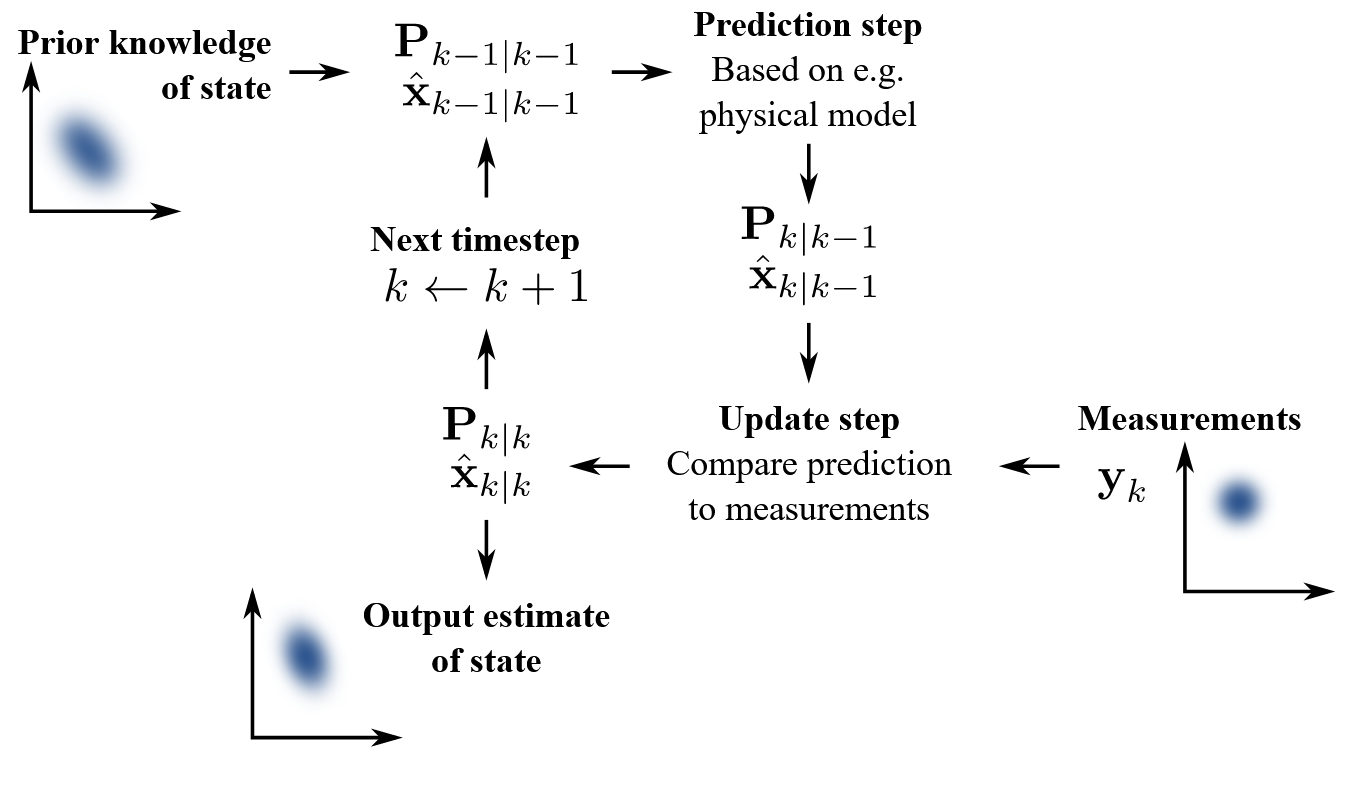
\includegraphics[width=\textwidth]{../../Images/Étapes du filtre de Kalman avec équations.png}
	\caption{Schematic representation of the Kalman filter prediction/correction cycle. At each time step, the previous PDF $\mathcal{N}\left(\hat{x}_{k-1|k-1}, P_{k-1|k-1}\right)$ is propagated through the state transition model (prediction), then updated using the new observation $z_k$ (correction). Each ellipsoid represents a confidence region associated with its corresponding Gaussian density.}\label{fig:Kalman_filter}
\end{figure}

\begin{algorithm}[ht]
	\begin{algorithmic}
	\State{$\hat{x}_{k|k-1}=F_k\:\hat{x}_{k-1|k-1}+b_k^{(e)}$}\Comment{State prediction}
	\State{$P_{k|k-1}=F_k\:P_{k-1|k-1}\:F_k^\top+Q_k$}\Comment{Covariance prediction}
	\State{}
	\State{$y_k=z_k-\left(H_k\:\hat{x}_{k|k-1}+b_k^{(o)}\right)$}\Comment{Innovation}
	\State{$S_k=H_k\:P_{k|k-1}\:H_k^\top+R_k$}\Comment{Innovation covariance}
	\State{$K_k=P_{k|k-1}\:H_k^\top\:S_k^{-1}$}\Comment{Kalman gain}
	\State{$\hat{x}_{k|k}=\hat{x}_{k|k-1}+K_k\:y_k$}\Comment{State correction}
	\State{$P_{k|k}=(I-K_k\:H_k)\:P_{k|k-1}$}\Comment{Covariance correction}
	\end{algorithmic}\caption{Kalman Filter}\label{alg:Kalman_filter}
\end{algorithm}

\begin{remark}[Precomputation of gains]
	Under the assumptions of \eqref{eq:Kalman_assumptions}, the matrices $P_{k|k-1}$, $K_k$ and $P_{k|k}$ depend only on the system matrices $F_k$, $H_k$, $Q_k$, $R_k$ and the initial covariance $P_0$, but not on the observations $z_k$. They can therefore be computed offline before any measurement is received.
\end{remark}

\subsubsection{Joseph's Formula}

In finite-precision arithmetic, the standard update $P_{k|k}=(I-K_k\:H_k)\:P_{k|k-1}$ may lose symmetry or positive definiteness due to rounding errors. Joseph's formula gives an alternative way to compute $P_{k|k}$ while ensuring that this property remains numerically satisfied:
\begin{equation}
	\begin{aligned}
	P_{k|k}&=(I-K_k\:H_k)\:P_{k|k-1}\\
	&=(I-K_k\:H_k)\:P_{k|k-1}-K_k\:S_k\:K_k^\top+K_k\:S_k\:K_k^\top\\
	&=(I-K_k\:H_k)\:P_{k|k-1}-(P_{k|k-1}\:H_k^\top\:S_k^{-1})\:S_k\:K_k^\top+K_k\:(H_k\:P_{k|k-1}\:H_k^\top+R_k)\:K_k^\top\\
	&=(I-K_k\:H_k)\:P_{k|k-1}-P_{k|k-1}\:H_k^\top\:K_k^\top+K_k\:H_k\:P_{k|k-1}\:H_k^\top\:K_k^\top+K_k\:R_k\:K_k^\top\\
	&=(I-K_k\:H_k)\:P_{k|k-1}-(I-K_k\:H_k)\:P_{k|k-1}\:H_k^\top\:K_k^\top+K_k\:R_k\:K_k^\top\\
	&=(I-K_k\:H_k)\:P_{k|k-1}(I-K_k\:H_k)^\top+K_k\:R_k\:K_k^\top\\
	\end{aligned}
\end{equation}

Under this more robust form, $P_{k|k}$ is SPD as the sum of two SPSD matrices, the second of which is strictly positive definite.

\subsection{Extended Kalman Filter}

The hypothesis that the evolution and observation functions are affine in $x_k$ is often too restrictive in practice. The extended Kalman filter (EKF) relaxes this assumption by locally linearising $f_k$ and $h_k$ around the current state estimate via a first-order Taylor expansion.

Let $m,n\in\mathbb{N}^*$, let $f:\mathbb{R}^n\to\mathbb{R}^m$ be differentiable at some $a\in\mathbb{R}^n$. $f$ admits the following first-order expansion:
\begin{equation}
	\forall x\in\mathbb{R}^n,\:f(x)=f(a)+J_f(a)\:(x-a)+o(\|x-a\|_2)\label{eq:first_order_expansion}
\end{equation}
where $J_f(a)\in\mathcal{M}_{m,n}(\mathbb{R})$ is the Jacobian matrix of $f$ evaluated at $a$, and defined as:
\begin{equation}
	J_f\triangleq\frac{\partial f}{\partial x}=\begin{bmatrix}
	\dfrac{\partial f^{(1)}}{\partial x^{(1)}}&\cdots&\cdots&\dfrac{\partial f^{(1)}}{\partial x^{(n)}}\\
	\vdots&\ddots&\ddots&\vdots\\
	\dfrac{\partial f^{(m)}}{\partial x^{(1)}}&\cdots&\cdots&\dfrac{\partial f^{(m)}}{\partial x^{(n)}}
	\end{bmatrix}
\end{equation}
and $f^{(i)}$ and $x^{(j)}$ respectively denote the $i$-th and $j$-th component of $f$ and $x$.

Assuming that $f_k$ and $h_k$ are differentiable along the state trajectory, we can apply the first-order expansion \eqref{eq:first_order_expansion} to the evolution and observation model. Successive linearisations at each time step can then be used to apply the Kalman filter equations locally. The resulting algorithm is given by \Cref{alg:EKF}.

\begin{algorithm}[ht]
	\begin{algorithmic}
	\State{$\tilde{F}_k=J_{f_k}(\hat{x}_{k-1|k-1})$}\Comment{Evolution Jacobian}
	\State{$\hat{x}_{k|k-1}=f_k(\hat{x}_{k-1|k-1})+b_k^{(e)}$}\Comment{State prediction}
	\State{$P_{k|k-1}=\tilde{F}_k\:P_{k-1|k-1}\:\tilde{F}_k^\top+Q_k$}\Comment{Covariance prediction}
	\State{}
	\State{$\tilde{H}_k=J_{h_k}(\hat{x}_{k|k-1})$}\Comment{Observation Jacobian}
	\State{$y_k=z_k-\left(h_k(\hat{x}_{k|k-1})+b_k^{(o)}\right)$}\Comment{Innovation}
	\State{$S_k=\tilde{H}_k\:P_{k|k-1}\:\tilde{H}_k^\top+R_k$}\Comment{Innovation covariance}
	\State{$K_k=P_{k|k-1}\:\tilde{H}_k^\top\:S_k^{-1}$}\Comment{Kalman gain}
	\State{$\hat{x}_{k|k}=\hat{x}_{k|k-1}+K_k\:y_k$}\Comment{State correction}
	\State{$P_{k|k}=(I-K_k\:\tilde{H}_k)\:P_{k|k-1}$}\Comment{Covariance correction}
	\end{algorithmic}\caption{Extended Kalman Filter}\label{alg:EKF}
\end{algorithm}

While less restrictive than the standard Kalman filter, the EKF is suboptimal for three reasons:
\begin{itemize}
	\item First, $f_k$ and $h_k$ must be differentiable along the state trajectory, which excludes discontinuous or piecewise-defined models.
	\item Second, the linearisation in \eqref{eq:first_order_expansion} neglects higher-order terms of the Taylor expansion, which introduces an approximation error that grows with the degree of nonlinearity of $f_k$ and $h_k$. This error increases over time as it propagates through the equations of the Kalman filter due to the sequential formulation.
	\item Finally, it relies on Gaussian assumptions, and thus fails to handle multimodal or heavy-tailed distributions as its affine counterpart.
\end{itemize}

\subsection{Other Suboptimal Kalman Filters}

\subsubsection{Iterative EKF}

The iterative EKF (IEKF) improves upon the EKF correction step by iteratively re-linearising $h_k$ around successive state estimates within the same measurement update. The prediction step is identical to that of the EKF. Starting from the initialisation $\hat{x}_{k|k}^{(0)}=\hat{x}_{k|k-1}$, the IEKF iterates:
\begin{align}
	\tilde{H}_k^{(i)}&=J_{h_k}\left(\hat{x}_{k|k}^{(i-1)}\right)\\
	y_k^{(i)}&=z_k-\left(h_k\left(\hat{x}_{k|k}^{(i-1)}\right)+b_k^{(o)}\right)\\
	S_k^{(i)}&=\tilde{H}_k^{(i)}\:P_{k|k-1}\left(\tilde{H}_k^{(i)}\right)^\top\!+R_k\\
	K_k^{(i)}&=P_{k|k-1}\left(\tilde{H}_k^{(i)}\right)^\top\left(S_k^{(i)}\right)^{-1}\\
	\hat{x}_{k|k}^{(i)}&=\hat{x}_{k|k-1}+K_k^{(i)}\:\left(y_k^{(i)}-\tilde{H}_k^{(i)}\:\left(\hat{x}_{k|k-1}-\hat{x}_{k|k}^{(i-1)}\right)
	\right)
\end{align}
until convergence. Typically, the chosen stopping criterion is:
\begin{equation}
	\left\|\hat{x}_{k|k}^{(i)}-\hat{x}_{k|k}^{(i-1)}\right\|_2\leq\varepsilon
\end{equation}
for some $\varepsilon>0$. To prevent infinite iterations, a maximum number of steps is also usually given. The corrected state is defined after convergence as:
\begin{equation}
	\hat{x}_{k|k}=\hat{x}_{k|k}^{(i_{\max})}
\end{equation}
and its corresponding covariance matrix is computed as:
\begin{equation}
	P_{k|k}=\left(I-K_k^{(i_{\max})}\:\tilde{H}_k^{(i_{\max})}\right)\:P_{k|k-1}
\end{equation}
where $i_{\max}$ denotes the final value of $i$ after convergence.

The IEKF is thus very similar to the standard single-step EKF, with the difference that the correction step is performed more than once per time step. It is equivalent to performing a Gauss-Newton descent on the posterior density estimation problem, and converges to the MAP estimator under Gaussian assumptions.

\subsubsection{Higher-Order EKF}

The second-order EKF (SO-EKF) extends the linearisation \eqref{eq:first_order_expansion} to include second-order terms via the Hessians of $f_k$ and $h_k$, reducing the approximation error for highly nonlinear models. However, it requires computing and storing the Hessian matrices of $f_k$ and $h_k$ at each time step, making it computationally prohibitive in high dimensions. In practice, the unscented Kalman filter, presented below, achieves comparable accuracy through sigma-point propagation without explicit Hessian computation, and is generally preferred.

\subsubsection{Unscented Kalman Filter}

\textbf{TODO}
